\documentclass[12pt]{article} %Font Size 12 and Scientific Journal Style

%FONT STYLES - NEW TIMES ROMAN
%\usepackage{times}
%\usepackage{mathptmx}
\usepackage{newtxtext,newtxmath}

%FONT COLOUR
\usepackage{xcolor} %Font colour package
\color{black} %Set to black

%IMAGES
\usepackage{graphicx} %Images Package
\usepackage[small]{caption} %Figure Caption Package
\usepackage{float} %Force Image Placement with [H]
\graphicspath{ {./images/} } %Image File Directory
\captionsetup{font=footnotesize} %Set Figure Caption Font Size
\usepackage{placeins} % \FloatBarrier

%MATHS
\usepackage{amsfonts} %Number Set Symbols
\usepackage{amsmath} %Align Equations Package
	%function so '\\' doesn't label equation on that line
	%\makeatletter
	%\def\Let@{\def\\{\notag\math@cr}}
	%\makeatother

%UNITS
\usepackage{siunitx} %Standard Form Numbers Package

%PAGE LAYOUT
\usepackage{secdot} %Fullstop after section number package
\sectiondot{subsection} %Dot subsection numbers too
\pagestyle{plain} %Clear Header With Page Number In Footer
\numberwithin{equation}{subsection} %Correct equation numbering
\usepackage[top=2.54cm, bottom=2.54cm, left=2.75cm, right=2.75cm]{geometry}
% Set margin sizes
%\setlength{\parindent}{0cm} %Set paragraph indentation
%\linespread{1.2} %Set line spacing

%TABELS
\usepackage{array} %Table Package

%REFERENCING
%\usepackage{natbib} %Harvard referencing Package %Harvard Referencing (use \bibliographystyle{agsm})
\usepackage{cite} %IEEE Referencing Package (Use \bibliographystyle{ieeetr})
 	% webpage referencing
	\usepackage[hyphens]{url}
	\usepackage[breaklinks=true]{hyperref}

%COVER PAGE COMMAND
\newcommand{\makecover}[8]{
\thispagestyle{empty}
\setcounter{page}{0}\vskip 24pt
\begin{center}~\vskip 0.6in \LARGE{\bf {#1}}\vskip 12pt \normalsize{\textit{#2} and \textit{#3}}\vskip 6pt
\textit{#4} and \textit{#5} \vskip 24pt School of Physics and Astronomy\vskip 6pt The University of Manchester\vskip 24pt {#6} Year \\Theory Computing Project Report\vskip 24pt {#7}\vskip 36pt \end{center}\vskip 80pt
\section*{Abstract}
{#8}
\newpage}
%END OF COVER PAGE COMMAND

%IMAGE COMMAND
%\begin{figure}[H]
%   \centering
%	\captionsetup{justification=centering}
%	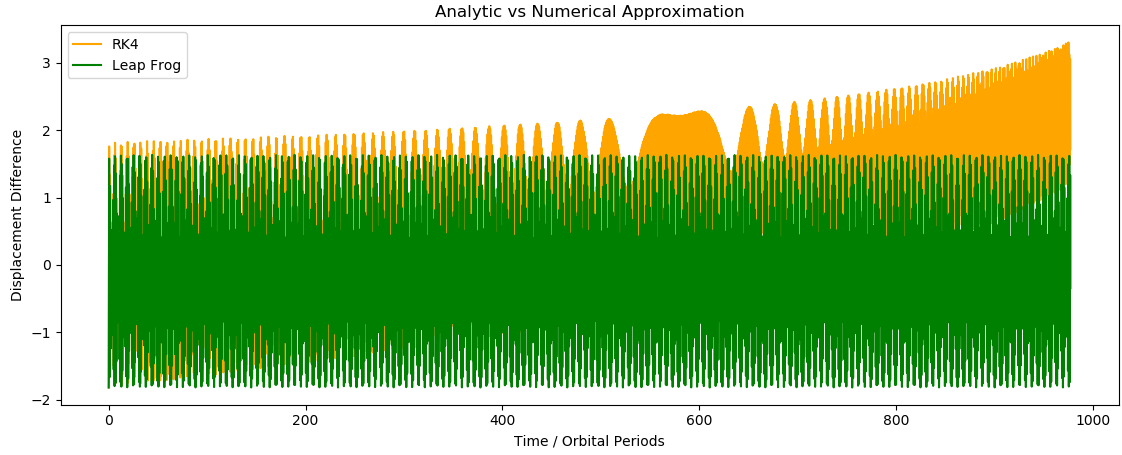
\includegraphics[scale=0.6]{images/anavsLeapvsRK4v2.png}
%	\caption{hello}
%	\label{fig:anaVSleap}
%	\end{figure}

%BEGIN
\begin{document}
\sisetup{mode=text,
	detect-all}
\makecover
{The classical H\textsubscript{2}\textsuperscript{+} ion}
{Christopher Kitching}
{Elanor Harrington}
{10134621}
{10134324}
{Second}
{Apr 2019}
{The aim of this project was to use purely classical physics to simulate the orbital motion of the positive molecular hydrogen ion, H\textsubscript{2}\textsuperscript{+}. This was achieved by using various numerical integration techniques, namely the leapfrog and Runge-Kutta 4\textsuperscript{th} order methods, to solve Newton's equations of motion. The numerical accuracy of these integration techniques was considered throughout. The simulations increased in complexity; beginning with a simple two-body model of the ion, up to the general three-body model. Where possible, comparisons with the analytic solution were explored.}

\pagenumbering{arabic} %Set page numbers style
\setcounter{page}{2} %Begin numbering at page 2

\section{Introduction}

The molecular hydrogen ion, H\textsubscript{2}\textsuperscript{+}, consists solely of two positively charged protons and a single negatively charged electron. The motivation to study the H\textsubscript{2}\textsuperscript{+} ion originates from the fact that it only has one electron. This means that we do not need to account for additional electron-electron repulsion, making molecular hydrogen the simplest molecule that can be formed. Consequently, it is relatively straightforward to solve the equations of motion for this system. Models for more complicated problems, such as the N-body problem, can then be built from models of the H\textsubscript{2}\textsuperscript{+} ion. Such models have a wide range of applications in many fields where it is difficult to observe processes on the atomic level; for example, to study the physical properties of nanotechnology in material science \cite{wang2012molecular}, or to investigate the motion of macromolecules in biological systems \cite{mccammon1977dynamics}. This report ultimately explores the motion of an electron acted upon by the electrostatic field of two protons which are also free to move in space, i.e the three-body problem. This was achieved through molecular dynamics; a computational simulation method used to study the motion of particles by numerically solving Newton's equations of motion \cite{alder1959studies}. The two numerical integrators used were the Runge-Kutta 4\textsuperscript{th} order method, otherwise known as RK4, and the leapfrog method, with their numerical accuracy and suitability for the problem being explored in detail. On route to the general solution, the simpler scenarios of one and two protons at fixed positions were investigated. Note that throughout this report all constants have been set to 1 for simplicity. This also allows the problem to be easily extended to consider other inverse square-law forces, such as gravitation.

\section{Theory}

\subsection{Analytic solution} \label{sec: analytic}
\FloatBarrier

For the motion of a single particle being acted upon by a central force, the formal equation of its orbit is given by \cite[p; 28]{fetter2003theoretical}
\begin{equation}
    r=\frac{L^{2}}{\mu \alpha (1+\epsilon cos(\phi))}, \label{eq: conic}
\end{equation}
where $\phi$ is the angle that $r$, the orbital radius, makes with the the point of closest approach, $L$ is the angular momentum, $\mu$ is the reduced mass of the system and $\alpha$ is a constant whose value is dependent on the force field. In this purely electrostatic case $\alpha$ is defined by \cite[p; 7]{huray2011maxwell}
\begin{equation}
    \alpha=k\textsubscript{e}q\textsubscript{1}q\textsubscript{2}, \label{eq: coulomb}
\end{equation}
where $q\textsubscript{1}$ and $q\textsubscript{2}$ are the signed magnitudes of the charges of the particles involved in the motion and $k\textsubscript{e}$ is Coulomb's constant which is approximately equal to \SI{9e9}{N m^{2} C^{-2}} \cite[p; 7]{huray2011maxwell}. $\epsilon$ is the eccentricity of the orbit, given by \cite[p; 28]{fetter2003theoretical}
\begin{equation}
    \epsilon=\left(1+\frac{2L^{2}}{\mu \alpha^{2}}E\right)^{\frac{1}{2}}, \label{eq: eccen} 
\end{equation}
where $E$ is the total energy of the system. Equation (\ref{eq: conic}) describes an orbit that is a conic section \cite[p; 28]{fetter2003theoretical}, so by changing the initial conditions of the system we can manipulate the value of $\epsilon$, or equivalently $E$, in order to alter the shape of the orbit. The parameter values required to obtain the main orbital shapes are summarised in Table \ref{tab: orbitShapes}.
	\begin{table}[h]
	\begin{center}
	\begin{tabular}{|c|c|c|}
	\hline
	\textbf{Orbital Shape}&\textbf{Eccentricity ($\epsilon$)}&\textbf{Total Energy ($E$)}\\
	\hline
	Circular&$\epsilon=0$&$E=-\frac{\mu \alpha^{2}}{2L^{2}}$\\
	Elliptical&$0<\epsilon<1$&$E<0$\\
	Parabolic&$\epsilon=1$&$E=0$\\
	Hyperbolic&$\epsilon>1$&$E>0$\\
	\hline
	\end{tabular}
	\captionsetup{justification=centering}
	\caption{A table showing the main orbital shapes of a particle in a central force field, along with the required parameter values to achieve such orbits \cite{curtis2013orbital}.}
	\label{tab: orbitShapes}
	\end{center}
	\end{table} \par

\FloatBarrier
\subsection{Computational methods} \label{sec: Computational Methods}
The two methods of numerical integration used were the 2\textsuperscript{nd} order leapfrog method, and the 4\textsuperscript{th} order Runge-Kutta method. Both of these methods are frequently used in the simulation of classical dynamical systems to determine the motion of a particle in a force field by solving differential equations of the form
\begin{equation}
    \frac{d^{2}x}{dt^{2}}=F(x), \label{eq: 2ndDeriv}
\end{equation}
where $x$ is the position of the particle, $t$ is the time and $F$ is a function proportional to the force. Both these methods work by taking some initial conditions and updating their values at successive time-steps, however they achieve this in different ways. \par
For the leapfrog method, the equations for updating the position and velocity can be written in the 'kick-drift-kick' form \cite[p; 5]{dehnen2011n}
\begin{equation}
    \begin{aligned}
    a_{i}&=F(x_{i}), \\
    v_{i+\frac{1}{2}}&=v_{i}+a_{i}\frac{h}{2}, \\
    x_{i+1}&=x_{i}+v_{i+\frac{1}{2}}h, \\
    v_{i+1}&=v_{i+\frac{1}{2}}+a_{i+1}\frac{h}{2},
    \end{aligned}
\end{equation}
where $v$ is the velocity, $a$ is the acceleration and $h$ is the size of the time-step which we require to be greater than zero. The subscripts on the variables denote the step at which the variable is evaluated.  \par
For the RK4 method we first re-cast equation (\ref{eq: 2ndDeriv}) as an initial value problem of the following form
\begin{equation}
    \begin{aligned}
    y&=\frac{dx}{dt}, \\
    f(y,t)&=\frac{dy}{dt}, \\
    y(t_{0})&=y_{0},
    \end{aligned}
\end{equation}
where $y$ is some unknown function of arbitrary size that we wish to approximate, $t_{0}$ is the initial time and $y_0$ are the initial conditions of the system. We then define \cite[p; 328]{suli2003introduction}
\begin{equation}
    \begin{aligned}
    k_{1}&=hf\left(t_{i},y_{i}\right), \\
    k_{2}&=hf\left(t_{i}+\frac{h}{2},y_{i}+\frac{k_{1}}{2}\right), \\
    k_{3}&=hf\left(t_{i}+\frac{h}{2},y_{i}+\frac{k_{2}}{2}\right), \\
    k_{4}&=hf\left(t_{i}+h,y_{i}+k_{3}\right),
    \end{aligned}
\end{equation}
where $k_{1}$,$k_{2}$,$k_{3}$ and $k_{4}$ are increments based on the slope of $y$ at various intervals of $h$. These parameters can then be used to update $y$ and $t$ using \cite[p; 328]{suli2003introduction} 
\begin{equation}
    \begin{gathered}
    y_{i+1}=y_{i}+\frac{1}{6}(k_{1}+2k_{2}+2k_{3}+k_{4}), \\
    t_{i}=t_{i}+h.
    \end{gathered} \label{eq: RK4updated}
\end{equation}
Equation (\ref{eq: RK4updated}) gives greater weight to the $k_{2}$ and $k_{3}$ terms since the slope at the mid-point should give a better estimate of the actual slope. Note that if $f$ is independent of $y$ the problem becomes a simple integral and the RK4 method reduces to Simpson's rule \cite[p; 328]{suli2003introduction}. \par
As the leapfrog method is a 2\textsuperscript{nd} order method, the total accumulated error is of order $\mathcal{O}$($h^{2}$), whereas the error of RK4, being a 4\textsuperscript{th} order method, is of order $\mathcal{O}$($h^{4}$) \cite{sandvik2015numerical}. We hence expect that RK4 will give a more accurate solution to the problem, although this comes at the expense of computation time. \par 
However, the main strength of leapfrog is that it is a symplectic algorithm, meaning that it does not suffer from energy drift, which is the gradual shift in the total energy of a closed system over long time periods \cite[p; 11]{young2014leapfrog}. This makes leapfrog the better numerical integrator when computing long term orbital dynamics. \par
The comparison between these two numerical integration methods and their properties is explored in more detail in sub-section \ref{subsec: numerical considerations}.

\section{Results and analysis} \label{Sec: Results and Analysis}
\FloatBarrier

\subsection{Two-body problem} \label{subsec: two-body}
The most simple system we can consider in orbital dynamics is that of an electron orbiting a single fixed proton. As discussed in sub-section \ref{sec: Computational Methods}, there are four main orbital shapes that can be obtained by varying the parameters $\epsilon$, or $E$, which are shown in Figure \ref{fig: combined plots}. Note that the plots in Figure \ref{fig: combined plots} have been generated using the leapfrog method, however RK4 will produce near identical plots for short term orbital dynamics such as this. \par
\begin{figure}[h]
    \centering
    \captionsetup{justification=centering}
	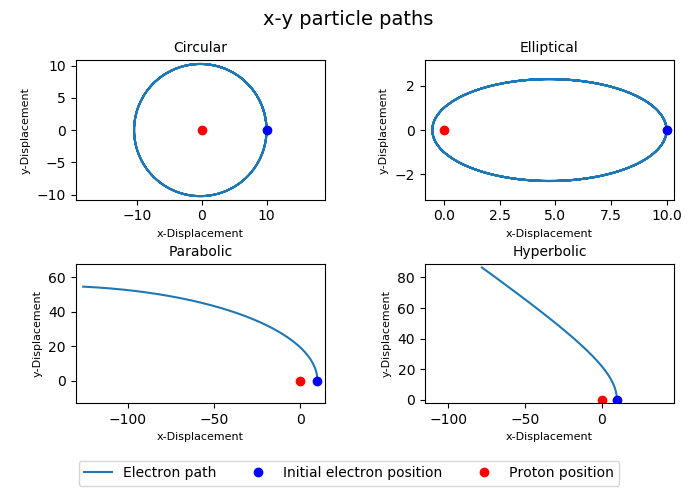
\includegraphics[scale=0.45]{images/combinedPlot3.png}
	\caption{Four subplots demonstrating the basic electron paths for an electron orbiting a single stationary proton, i.e the two-body problem.}
	\label{fig: combined plots}
	\end{figure}
	
\subsection{Numerical considerations} \label{subsec: numerical considerations}
Before moving onto the case of two protons the numerical limits of the model were considered. First of all, the optimum step-size to run the simulations was determined. Using a step-size that is too large produced inaccurate results, however extremely small step-sizes were computationally expensive. Figure \ref{fig: optimal step size} shows a plot of the average energy calculated numerically for Leapfrog and RK4 plotted against the step-size. It is clear that as the step-size decreases the numerical approximation of the energy approaches the true value in each case as the model becomes more accurate. It is usually desirable for the numerical energy to be in the range of 0.1-0.01\% of the true value; the 0.1\% boundaries are highlighted in Figure \ref{fig: optimal step size}. RK4 appears to reach this region before leapfrog, which is as expected given RK4 is a higher order method and so should be more accurate for a given step-size. Although leapfrog needs to run with a lower step-size, the algorithm itself has less steps, making it the less computationally expensive method overall. This method of considering energy convergence was employed throughout the project in order to determine a good step-size for any given initial condition. \par
\begin{figure}[h]
    \centering
    \captionsetup{justification=centering}
	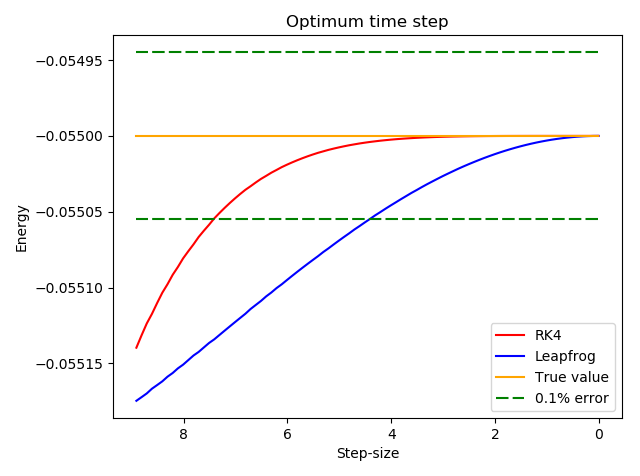
\includegraphics[scale=0.45]{images/optimalStepSize4.png}
	\caption{A plot showing the energy convergence to the initial energy value of two numerical integration methods, leapfrog and RK4, with step-size. Boundaries representing a 0.1\% difference from the true value have been highlighted.}
	\label{fig: optimal step size}
	\end{figure}
Another consideration that was investigated was the symplectic properties of the leapfrog method, which were discussed in sub-section \ref{sec: Computational Methods}. Figure \ref{fig: energy comparison} shows a plot of the total energy of the system against time for both methods. At large time periods the total energy as determined by RK4 begins to deviate from the true value. This energy drift makes RK4 a poor numerical integrator for modelling long term behaviour of the system.
\begin{figure}[h]
    \centering
    \captionsetup{justification=centering}
	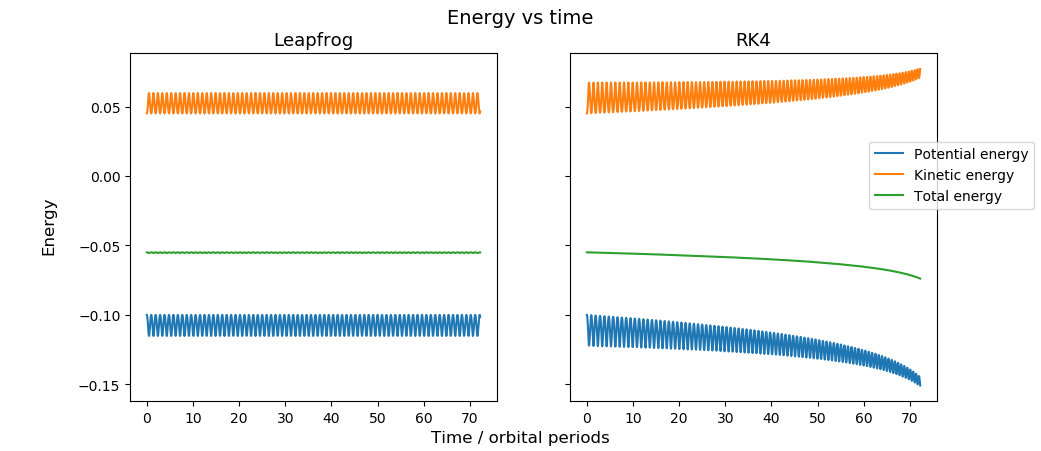
\includegraphics[scale=0.45]{images/energyComparison3.png}
	\caption{A plot showing the energy conservation of the system for two different numerical methods; leapfrog and RK4.}
	\label{fig: energy comparison}
	\end{figure}
A similar conclusion can be drawn from comparison between the numerical and analytic results. Figure \ref{fig: ana vs numeric} shows a plot of the difference in the average electron position between the analytic solution, as detailed in sub-section \ref{sec: analytic}, and the results of both numerical methods. It can be seen that over time the result of RK4 drifts away from the analytic solution whereas the leapfrog result will oscillate about the true value for all time, as a consequence of its symplectic nature \cite[p; 11]{young2014leapfrog}. \par
\begin{figure}[h]
    \centering
    \captionsetup{justification=centering}
	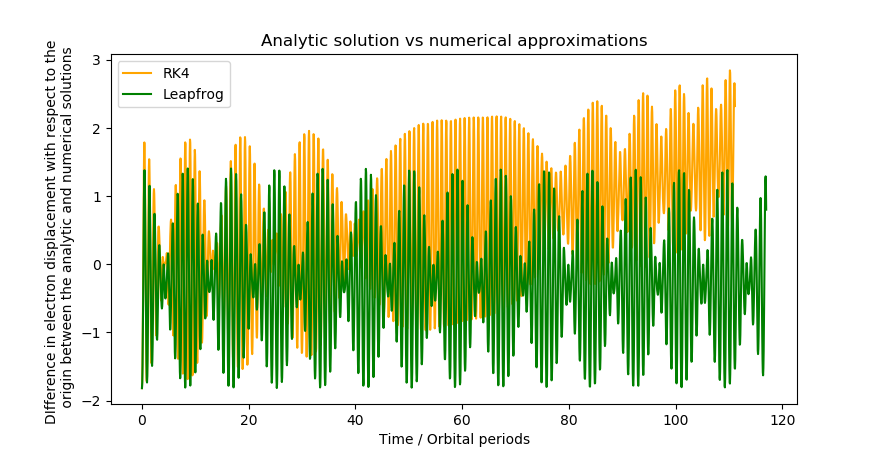
\includegraphics[scale=0.45]{images/anavsLeapvsRK4v4.png}
	\caption{A plot of the difference in the average electron displacement, with respect to the origin, between the analytic solution and the two numerical methods, leapfrog and RK4, for the two-body problem.}
	\label{fig: ana vs numeric}
	\end{figure}
The conclusion from all the numerical considerations discussed above is that for our purposes leapfrog was the more suitable numerical integrator, mainly due to our desire to analyse the system over long time periods. For this reason, the leapfrog method became the default choice going forward with this problem. \par

\subsection{Restricted three-body problem} \label{subsec: restricted three-body}
Adding an additional proton to the problem increases the complexity substantially. The limiting case of two stationary protons was considered first. \par
It is expected that if the initial conditions of the system are such that the proton separation is negligible compared to the electron displacement with respect to the origin, then its behaviour should approach that of the two-body problem detailed in sub-section \ref{subsec: two-body}. This property is highlighted in Figure \ref{fig: two-body convergence}, which shows the energy difference between the limiting and general case converging to zero as the ratio of initial electron displacement to proton separation increases. \par
\begin{figure}[h]
    \centering
    \captionsetup{justification=centering}
	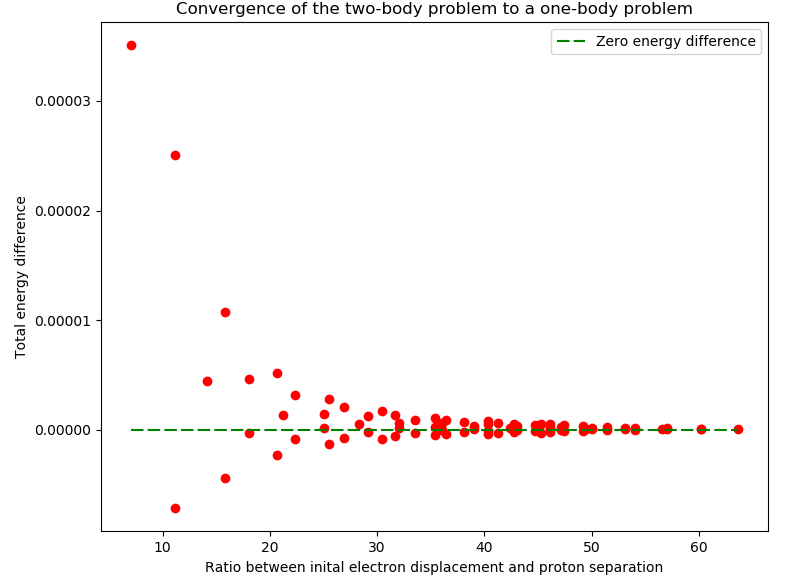
\includegraphics[scale=0.4]{images/twoBodyConvergence3.png}
	\caption{A plot of the difference in the total energy of the system between the two-body and three-body problem, against the ratio of initial electron displacement to proton separation.}
	\label{fig: two-body convergence}
	\end{figure}
There exists a variety of orbital shapes for an electron orbiting two protons. For the limiting case of the three-body problem, the majority of orbits are stable, i.e the electron remains bound to the atom. An intuitive orbit for the restricted case is a figure-eight pattern which is shown in Figure \ref{fig: stat protons}. The initial conditions used to generate this plot are used in all further analysis in order to allow for consistent comparisons between the various problems.
\begin{figure}[h]
    \centering
    \captionsetup{justification=centering}
	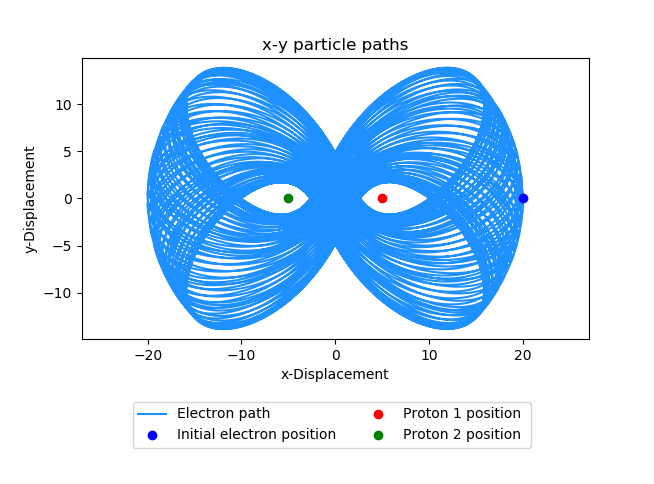
\includegraphics[scale=0.45]{images/statPath2.png}
	\caption{A plot showing an example orbit for the restricted three-body problem. In this case, the electron path takes the shape of a figure-eight pattern.}
	\label{fig: stat protons}
	\end{figure}


\subsection{Three-body problem} \label{subsec: three-body problem}

To generalize to the three-body problem the constraint of stationary protons was removed. Once this was allowed the system appeared to become unstable. Figure \ref{fig: mov protons} shows the particle paths produced for the general three-body problem when using the same initial conditions as those used to generate the figure-eight pattern for the restricted three-body problem in Figure \ref{fig: stat protons}. \par
\begin{figure}[h]
    \centering
    \captionsetup{justification=centering}
	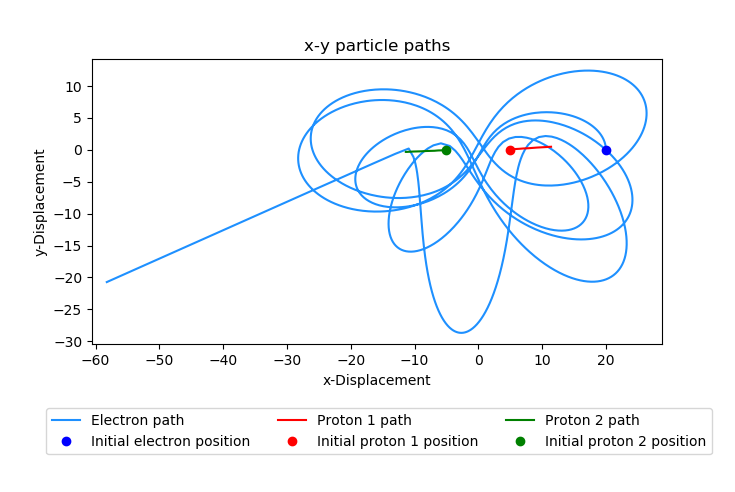
\includegraphics[scale=0.45]{images/movPath2.png}
	\caption{A plot showing the paths of particles for the general three-body case. The initial conditions are the same as that used to generate Figure \ref{fig: stat protons}}
	\label{fig: mov protons}
	\end{figure}
The general case of the three-body problem, as shown in Figure \ref{fig: mov protons}, seems to show the electron moving off to infinity after being slingshot by one of the protons. This problem occurred in the majority of orbits initially tested and was a surprising result as intuition suggests that it is physically unlikely that all initial conditions would give this end result. A more severe problem became apparent when the energy conservation was checked. 
\begin{figure}[h]
    \centering
    \captionsetup{justification=centering}
	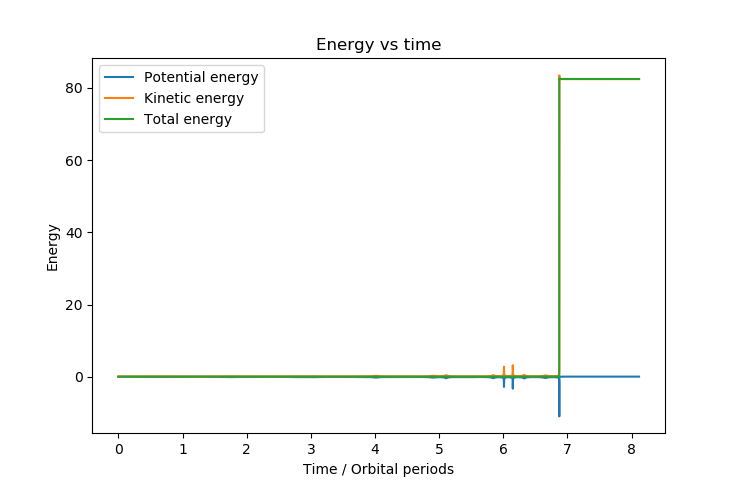
\includegraphics[scale=0.45]{images/unconservedEnergy2.png}
	\caption{A plot showing the energy for the three-body system. The total energy is not conserved for the entire motion.}
	\label{fig: unconserved energy} 
	\end{figure}
Figure \ref{fig: unconserved energy} shows that energy conservation is obeyed until the electron moves too close to one of the protons, at which point the total energy rapidly increases with time and conservation of energy is violated. This issue is often called 'exploding' and is caused when the time step is too large and propagates the position of the electron to be almost on top of one of the protons. This effectively gives an atomic collision, which our model is not built to handle, and as a consequence the energy conservation is violated \cite{kim2014issues}. \par
However, as mentioned in sub-section \ref{subsec: numerical considerations}, small time-steps are computationally expensive; even more so for long term motion. To get around this issue, a dynamical step-size was implemented, which scaled the step-size with respect to the acceleration of the proton. Consequently, when the electron was close to the proton, i.e. its acceleration was larger than average, the step-size would be dramatically reduced in order to increase the accuracy of the simulation. \par
This solution partially resolved the problem detailed above and we arrived at a more sensible result wherein the protons gradually repelled one another and the electron became bound to a single proton as shown in Figure \ref{fig: path variable time step}.
\begin{figure}[h]
    \centering
    \captionsetup{justification=centering}
	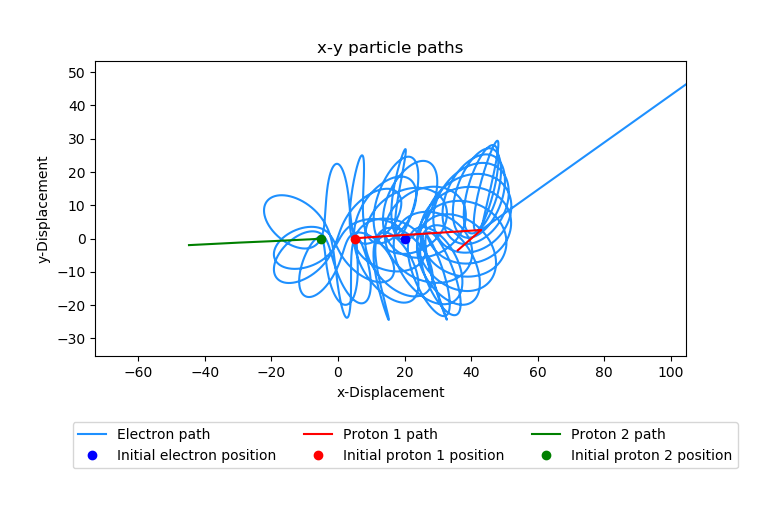
\includegraphics[scale=0.45]{images/pathVarTimeStep4.png}
	\caption{A plot showing the x-y path of the electron and the two protons for the three body case using a variable time-step. The same initial conditions as in Figure \ref{fig: mov protons} have been used.}
	\label{fig: path variable time step} 
	\end{figure}
Note however that eventually the electron and proton collide once more. This can again be corrected by using an even more accurate time-step, albeit at a large computational expense. Ultimately the problem is that the equations of motion for molecular dynamics are inherently chaotic, which means there exists an error in the simulation that grows exponentially with time and eventually overwhelms our numerical trajectories \cite{skeel2009makes}. This is unfortunately a numerical inaccuracy which can never be entirely eliminated. However, the more important result to note is that increasing the accuracy of the time-step made the orbit more stable. Assuming this trend holds, then the instability for a simulation with an infinitely small time-step would be due to the protons drifting apart. This instability was then investigated further by attempting to quantize it.
\begin{figure}[h]
    \centering
    \captionsetup{justification=centering}
	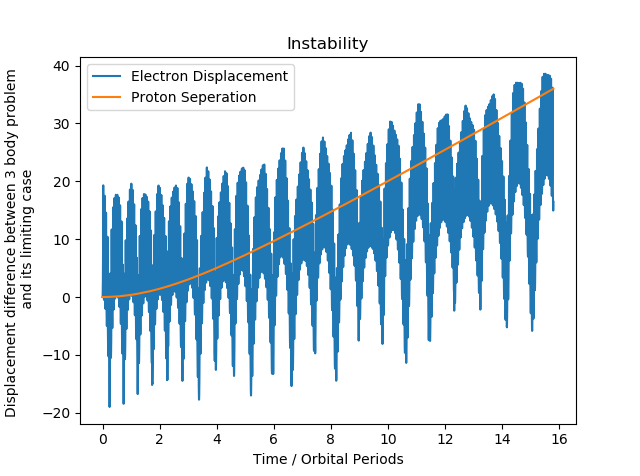
\includegraphics[scale=0.45]{images/instability2.png}
	\caption{A plot showing the proton separation and the electron displacement with respect to the origin in the case of the general three-body problem. The separation of the protons gradually increases as they repel each other, while the electron stays bound and orbits one of the protons.}
	\label{fig: instability} 
	\end{figure}
Figure \ref{fig: instability} shows such a quantization for the motion of the system before the inevitable atomic collision, where the separation of the protons increases over time while, in this case, the electron remains in orbit around one of the protons. This result is not a numerical error, rather an error in the model itself and the assumptions that were made. It has long been known that the classical model of atoms or molecules is incomplete. Particles such as electrons and protons cannot be treated as point like charges that have definite positions and momentum and so their orbits cannot be determined through purely geometrical arguments. We would instead have to consider the wavefunctions of the particles and solve Schr\"{o}dinger's equation \cite{schrodinger1926undulatory}. The first successful treatment of which, in the case of the H\textsubscript{2}\textsuperscript{+} ion, was done in 1927 by Danish physicist \O yvind Burrau \cite{burrau1927berechnung}.


\subsection{The three-body problem in 3-dimensions}
As an extension the generalization of the three-body problem to three-dimensional space was made. It was relatively straight forward to do this; requiring only an additional set of equations to account for the extra dimension. The addition of a new dimension allows for many more interesting scenarios. However, as we discovered in section \ref{subsec: three-body problem}, the system is still unstable. An example of this is demonstrated in Figure \ref{fig: 3D} which shows the particle paths in three-dimensions. As in Figure \ref{fig: path variable time step}, the protons gradually drift apart and the electron becomes locked in orbit with a single proton.	
\begin{figure}[h]
    \centering
    \captionsetup{justification=centering}
	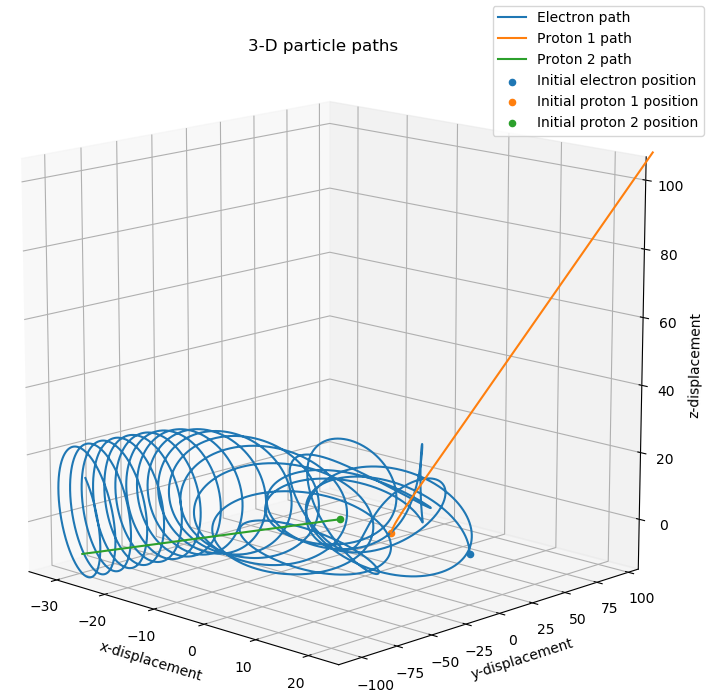
\includegraphics[scale=0.45]{images/3D2.png}
	\caption{A plot showing the particle paths of the individual particles that constitute the molecular hydrogen ion for the general three-body problem in three-dimensions.}
	\label{fig: 3D} 
	\end{figure}

\FloatBarrier
\section{Conclusion}
In this report we have compared two different numerical integrators, namely RK4 and leapfrog, for use in analyzing the motion of simple atoms and molecular ions. Ultimately, by considering total energy and comparison with the analytic solution, the leapfrog method was determined to be the more appropriate method mainly due to its symplectic nature. This numerical method was then employed to solve for the orbital motion of the constituent particles of the molecular hydrogen ion, given the initial conditions of instantaneous position and velocity. The simple two-body problem was solved first before the general three-body problem was eventually considered. It was then shown that the H\textsubscript{2}\textsuperscript{+} ion was unstable due to the protons gradually drifting apart over time. This behaviour was a limitation of the model, and although quantum mechanics is needed for a complete understanding, this is a different problem and our classical modelling still has many useful applications. Most notably, an extension to more involved problems, such as the N-body problem, can be made which allows for more complicated systems of molecules to be studied. The model could also be easily adapted to deal with other inverse-square law forces such as gravity; allowing study of the motion or formation of large scale stellar structures.

\section{Length and date}
The number of words in this document is 3444 \\
This document was submitted on 30/04/19.

\bibliographystyle{ieeetr}
\bibliography{./references}

\end{document}